%%%%%%%%%%%%%%%%%%%%%%%%%%%%%%%%%%%%%%%%%
% Beamer Presentation
% LaTeX Template
% Version 1.0 (10/11/12)
%
% This template has been downloaded from:
% http://www.LaTeXTemplates.com
%
% License:
% CC BY-NC-SA 3.0 (http://creativecommons.org/licenses/by-nc-sa/3.0/)
%
%%%%%%%%%%%%%%%%%%%%%%%%%%%%%%%%%%%%%%%%%

%----------------------------------------------------------------------------------------
%	PACKAGES AND THEMES
%----------------------------------------------------------------------------------------

\documentclass{beamer}

\mode<presentation> {

% The Beamer class comes with a number of default slide themes
% which change the colors and layouts of slides. Below this is a list
% of all the themes, uncomment each in turn to see what they look like.

%\usetheme{default}
%\usetheme{AnnArbor}
%\usetheme{Antibes}
%\usetheme{Bergen}
%\usetheme{Berkeley}
%\usetheme{Berlin}
%\usetheme{Boadilla}
%\usetheme{CambridgeUS}
%\usetheme{Copenhagen}
%\usetheme{Darmstadt}
%\usetheme{Dresden}
%\usetheme{Frankfurt}
%\usetheme{Goettingen}
%\usetheme{Hannover}
%\usetheme{Ilmenau}
%\usetheme{JuanLesPins}
%\usetheme{Luebeck}
%\usetheme{ClassyCharcoal}
%\usetheme{Malmoe}
%\usetheme{Marburg}
%\usetheme{Montpellier}
%\usetheme{PaloAlto}
%\usetheme{Pittsburgh}
\usetheme{Rochester}
%\usetheme{Singapore}
%\usetheme{Szeged}
%\usetheme{Warsaw}

% As well as themes, the Beamer class has a number of color themes
% for any slide theme. Uncomment each of these in turn to see how it
% changes the colors of your current slide theme.

%\usecolortheme{albatross}
%\usecolortheme{beaver}
%\usecolortheme{beetle}
%\usecolortheme{crane}
%\usecolortheme{dolphin}
%\usecolortheme{dove}
%\usecolortheme{fly}
%\usecolortheme{lily}
%\usecolortheme{orchid}
%\usecolortheme{rose}
%\usecolortheme{seagull}
%\usecolortheme{seahorse}
\usecolortheme{whale}
%\usecolortheme{wolverine}

%\setbeamertemplate{footline} % To remove the footer line in all slides uncomment this line
\setbeamertemplate{footline}[frame number] % To replace the footer line in all slides with a simple slide count uncomment this line

%\setbeamertemplate{navigation symbols}{} % To remove the navigation symbols from the bottom of all slides uncomment this line
}

\usepackage{mathtools}
\usepackage{subfig}
\usepackage{graphicx} % Allows including images
\graphicspath{{figures/pdf/}{figures/eps/}{figures/jpg/}}
\usepackage{booktabs} % Allows the use of \toprule, \midrule and \bottomrule in tables
\usepackage{algorithmic}
\usepackage{epstopdf}
\usepackage[T1]{fontenc}

\usepackage{float}
\newfloat{algorithm}{t}{lop}
\floatname{algorithm}{Algorithm}

\usepackage{accents}
\newcommand{\ubar}[1]{\underaccent{\bar}{#1}}

\usepackage{amssymb}
\usepackage{cleveref}

\setbeamercovered{transparent}
%\useoutertheme{infolines}
\beamertemplatenavigationsymbolsempty

\pgfdeclareimage[height=0.5cm]{logo}{ut2}
\logo{\pgfuseimage{logo}}

\usepackage{array}
\newcolumntype{L}[1]{>{\raggedright\let\newline\\\arraybackslash\hspace{0pt}}m{#1}}

\usepackage[labelsep=colon]
                %labelfont={sf,bf},
                %textfont=sf]
               {caption}

\newenvironment{figure*}%
{\begin{figure}}
{\end{figure}}

\pdfmapfile{+sansmathaccent.map}

%----------------------------------------------------------------------------------------
%	TITLE PAGE
%----------------------------------------------------------------------------------------

\title[WSN Localization through DS Theory]{Development of Novel Computational Algorithms for Localization in Wireless Sensor Networks through Incorporation of Dempster-Shafer Evidence Theory}

\author{Colin Elkin} % Your name
\institute[UT] % Your institution as it will appear on the bottom of every slide, may be shorthand to save space
{
Advisor and Committee Chair: Dr.~Vijay Devabhaktuni \\
Committee: Dr.~Mansoor Alam, Dr.~Richard Molyet, and Dr.~Hong Wang \\
\medskip
Department of Electrical Engineering and Computer Science \\
The University of Toledo, College of Engineering 
}
\date{July 9, 2015} % Date, can be changed to a custom date

\begin{document}

\begin{frame}
\titlepage % Print the title page as the first slide
\end{frame}

\begin{frame}
\frametitle{Overview} % Table of contents slide, comment this block out to remove it
\tableofcontents % Throughout your presentation, if you choose to use \section{} and \subsection{} commands, these will automatically be printed on this slide as an overview of your presentation
\end{frame}

%----------------------------------------------------------------------------------------
%	PRESENTATION SLIDES
%----------------------------------------------------------------------------------------

%------------------------------------------------
\section{Introduction} 
%------------------------------------------------

%------------------------------------------------

\begin{frame}
\frametitle{Wireless Sensor Network}
\begin{columns}[c]
\column{.45\textwidth} 
\includegraphics<1>[width=\textwidth]{frame3-1.eps}
\includegraphics<2>[width=\textwidth]{frame3-2.eps}
\includegraphics<3>[width=\textwidth]{frame3-3.eps}
\includegraphics<4>[width=\textwidth]{frame3-4.eps}
\column{.45\textwidth} 
\begin{itemize}
\item{Collection of small, interchangeable low-power devices that monitor sensory data}
\item\uncover<2->{Node responds to event and sends alert signal}
\item\uncover<3->{Anchor node reads measurements from all sensor nodes}
\item\uncover<4->{Data from anchor nodes are processed to locate the node}
\end{itemize}
\end{columns}
\end{frame}

\begin{frame}
\frametitle{Problem Statement}
\begin{columns}[c]
\column{.32\textwidth} 
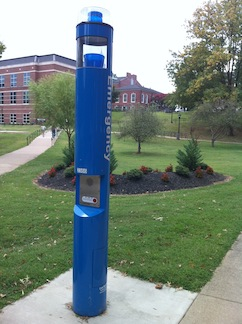
\includegraphics[width=.8\textwidth]{phone}
\column{.55\textwidth} 
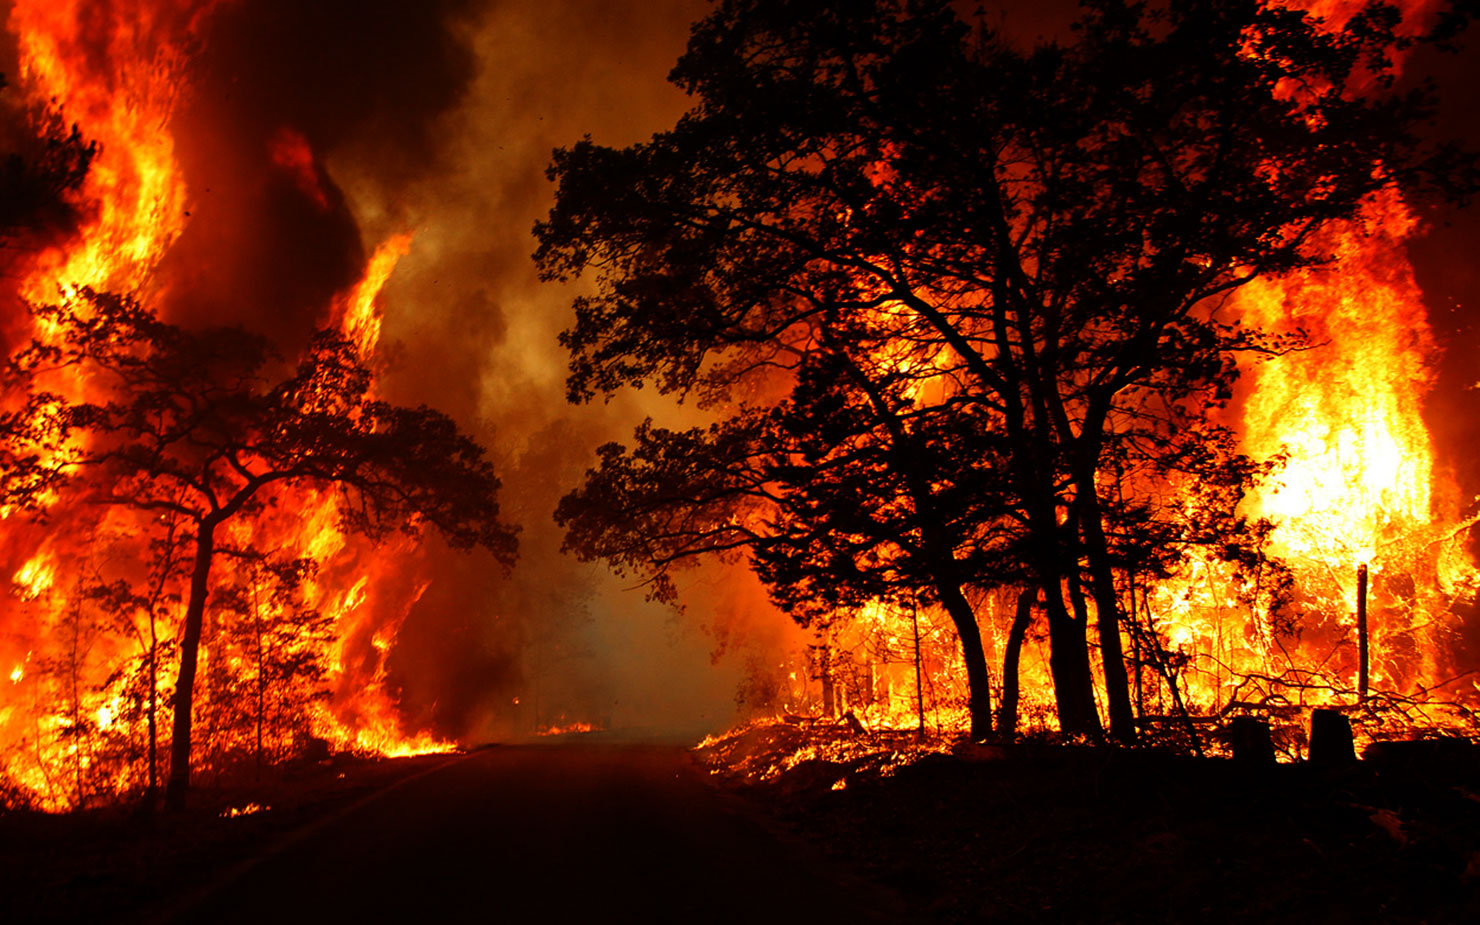
\includegraphics[width=\textwidth]{fire}
\end{columns}
\pause\begin{block}{Goals and Objectives of this Research}
{To develop new methods for finding a Node's location in a Wireless Sensor Network with both High Accuracy and Low Computational Cost}
\end{block}
\end{frame}

\begin{frame}
\frametitle{Established Localization Techniques}
\includegraphics<1>[width=.8\textwidth]{algs}
\includegraphics<2>[width=.8\textwidth]{algs1}
\end{frame}

\begin{frame}
\frametitle{Received Signal Strength (RSS)}
\begin{center}
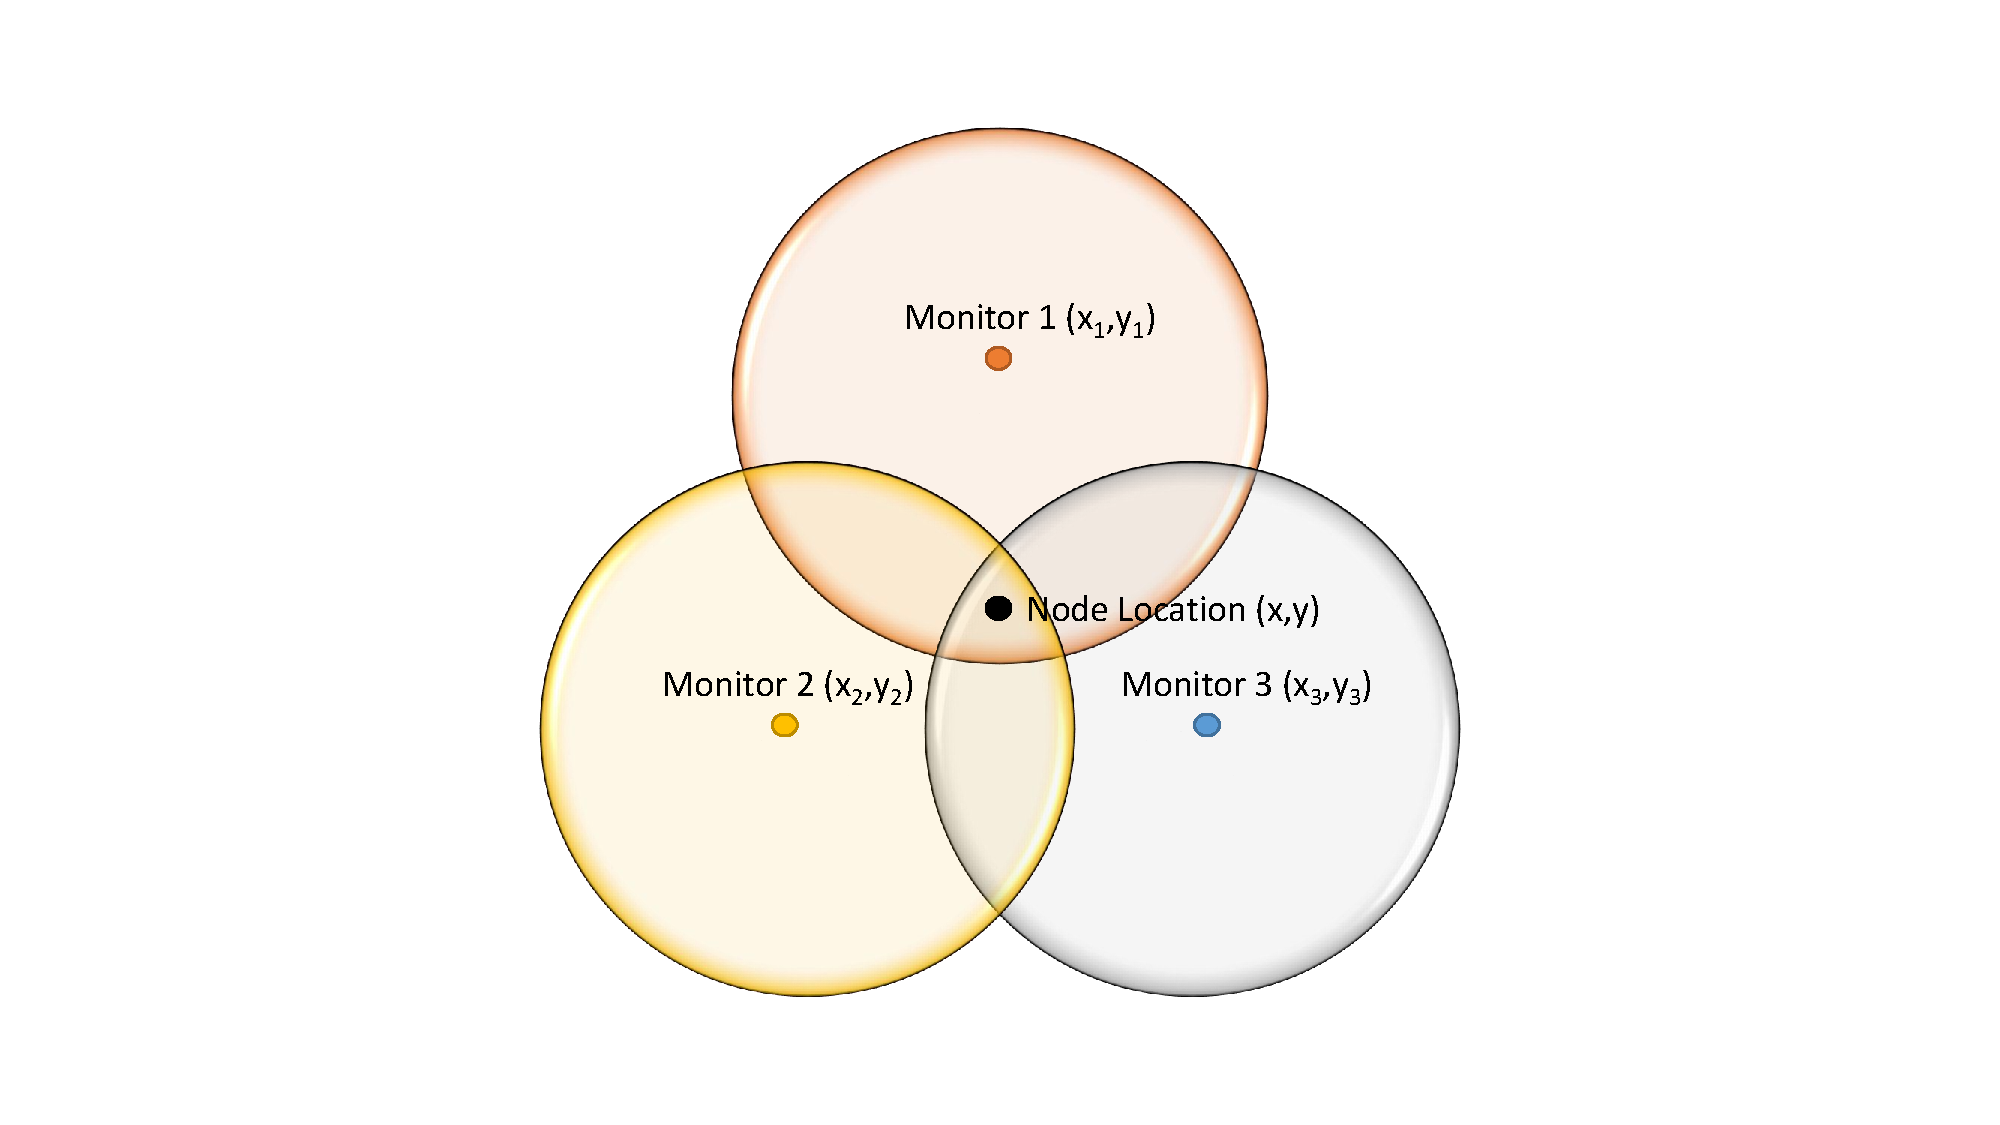
\includegraphics[width=.7\linewidth]{rss.pdf}
\end{center}
\begin{itemize}
\item{Defined as measured power or square of signal strength}
\item{Most vital property: RSS is inversely proportional to distance}
\item{Estimation done by trilateration}
\end{itemize}
\end{frame}

\begin{frame}
\frametitle{Angle of Arrival (AOA)}
\begin{center}
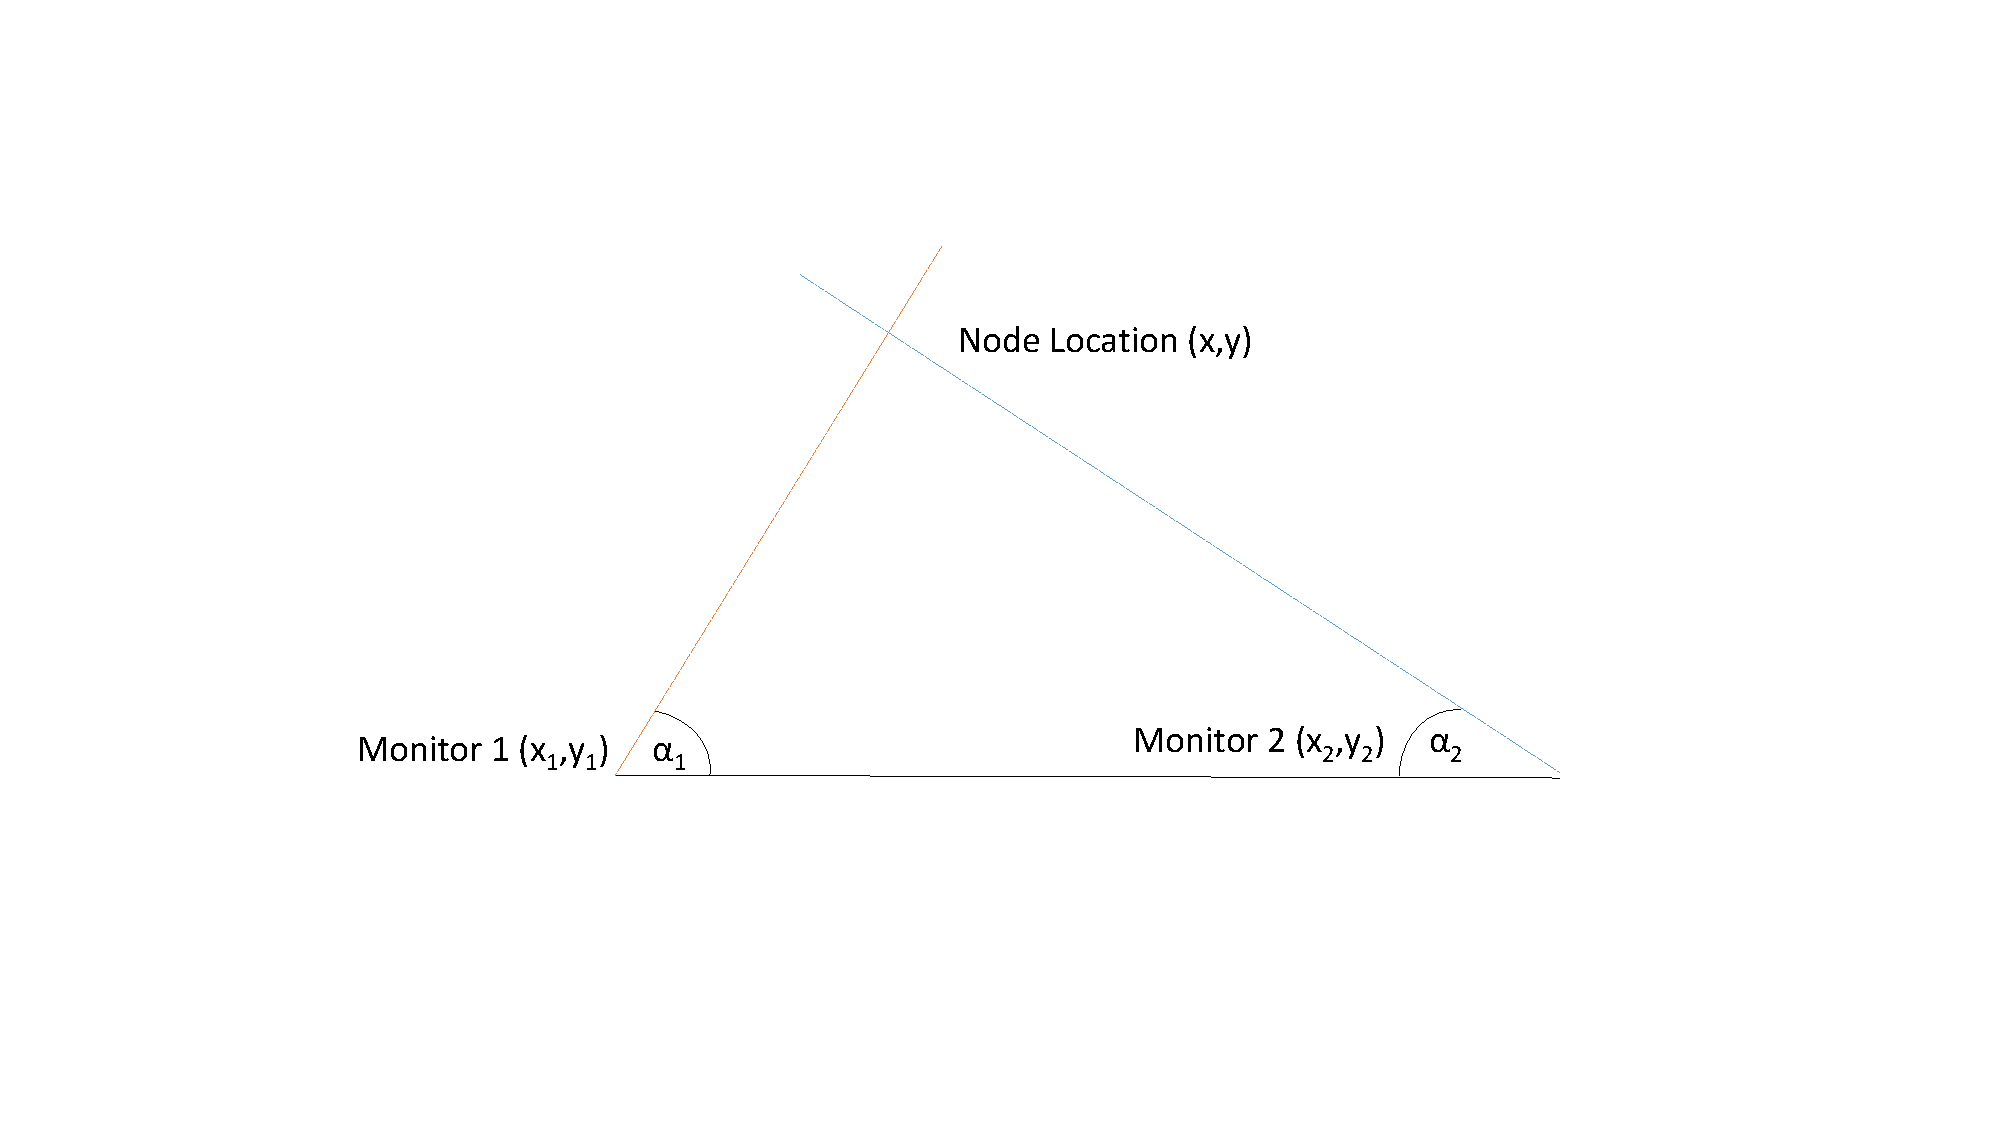
\includegraphics[width=.7\linewidth]{aoa.pdf}
\end{center}
\begin{itemize}
\item{Measures angles at 2+ receivers}
\item{Estimation done through triangulation}
\item{Based on TDOA measurements}
\end{itemize}
\end{frame}

\begin{frame}
\frametitle{Other Localization Techniques}
\begin{table}
\renewcommand{\arraystretch}{1.3}
\begin{tabular}{L{2cm} L{2cm} L{2cm} L{2cm}}
\toprule
\textbf{Technique} & \textbf{Overview} & \textbf{Advantages} & \textbf{Disadvantages} \\ 
\midrule
Genetic Algorithm (GA) & Evolutionary population of candidate solutions & Ideal for large-scale search problems & Premature convergence \\ 
Particle Swarm Optimization (PSO) & Based on particles and movements & Ideal for problems with real values & Expensive computational runtime \\ 
\bottomrule
\end{tabular}
\caption{Summary of global, biologically inspired localization techniques.}
\end{table}
\end{frame}

\begin{frame}
\frametitle{Overview of DS Theory}
\begin{center}
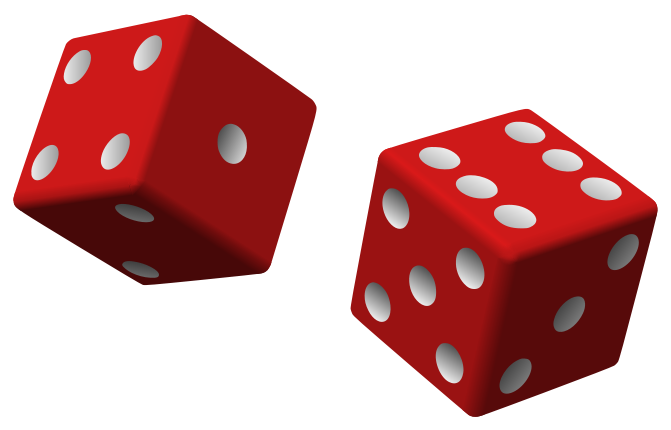
\includegraphics[width=.2\linewidth]{prob}
\end{center}
\begin{itemize}
\item{Divergence from Bayesian Probability}
\item{Based on concept of ignorance}
\item{Bayesian probability combines internal factors}
\item{DS Theory uses external factors}
\end{itemize}
\end{frame}

\begin{frame}
\frametitle{Example: Broken Chair}
\begin{table}
\begin{tabular}{l l }
\toprule
\textbf{Component} & \textbf{Failure Probability}\\
\midrule
Wheels & 60\% chance of breaking \\
Back & 20\% chance of falling apart \\
Arm Rests & 40\% chance of falling off \\
\bottomrule
\end{tabular}
\caption{Failure analysis of each chair component}
\end{table}

\pause
\begin{block}{Probability of Total Failure}
{$.6 \times .4 \times .2 = .048$ or 4.8\%}
\end{block}
\end{frame}

\begin{frame}
\frametitle{Example: Broken Chair}
\begin{table}
\begin{tabular}{l l l l}
\toprule
\textbf{Expert} & \textbf{Lower Bound} & \textbf{Upper Bound} & \textbf{Confidence}\\
\midrule
A & 11 & 18 & .4 \\
B & 14 & 21 & .4 \\
C & 10 & 20 & .2 \\
\bottomrule
\end{tabular}
\caption{Failure analysis by three experts}
\end{table}

\begin{itemize}
\pause\item{Expected Value Range of 100\% Failure: 12-19.6 Days}
\item{Most Plausible Time of 100\% Failure: 14 Days}
\item{Most Believable Time of 100\% Failure: 21 Days}
\end{itemize}
\end{frame}

\begin{frame}
\frametitle{Applications of and Motivations for DS Theory}
\begin{figure*}\centering
\subfloat[Failure Analysis \label{car}]
        {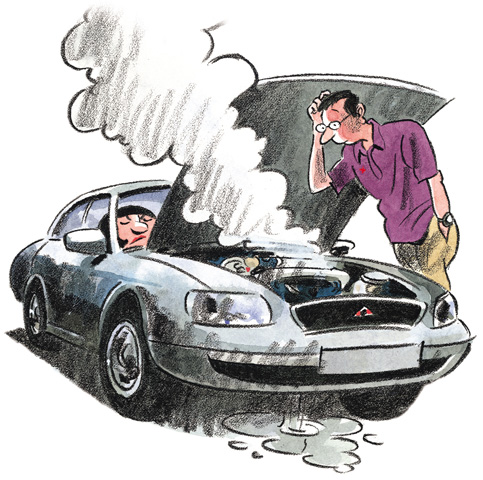
\includegraphics[width=0.22\textwidth]{broken_car}}
   % \hfill
\subfloat[Robot Sensor Fusion\label{robot}]
         {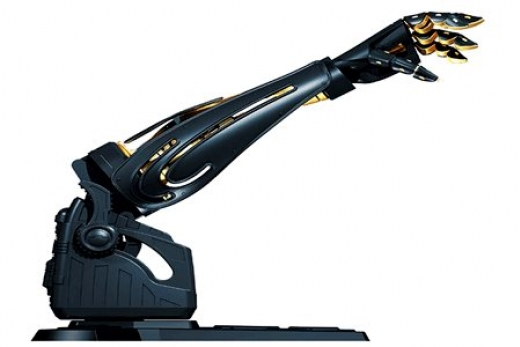
\includegraphics[width=0.22\textwidth]{robot}}
\subfloat[GPS/INS Data Fusion \label{gps}]
         {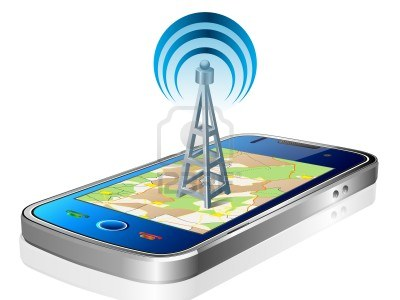
\includegraphics[width=0.22\textwidth]{gps}}
   % \hfill
\subfloat[Wireless Sensor Networks \label{wsn}]
        {
\includegraphics[width=0.22\textwidth]{wsn}}
    \label{apps}
    \end{figure*}
\begin{itemize}
\item{No need to train data}
\item{Fast and computationally efficient}
\end{itemize}
\end{frame}

\section{First Method: Expected Value}

\subsection{Introduction and Background}

\begin{frame}
\frametitle{First Proposed Algorithm}
\begin{itemize}
\item{Does the set of measurements belong to the county?}
\end{itemize}
\begin{center}
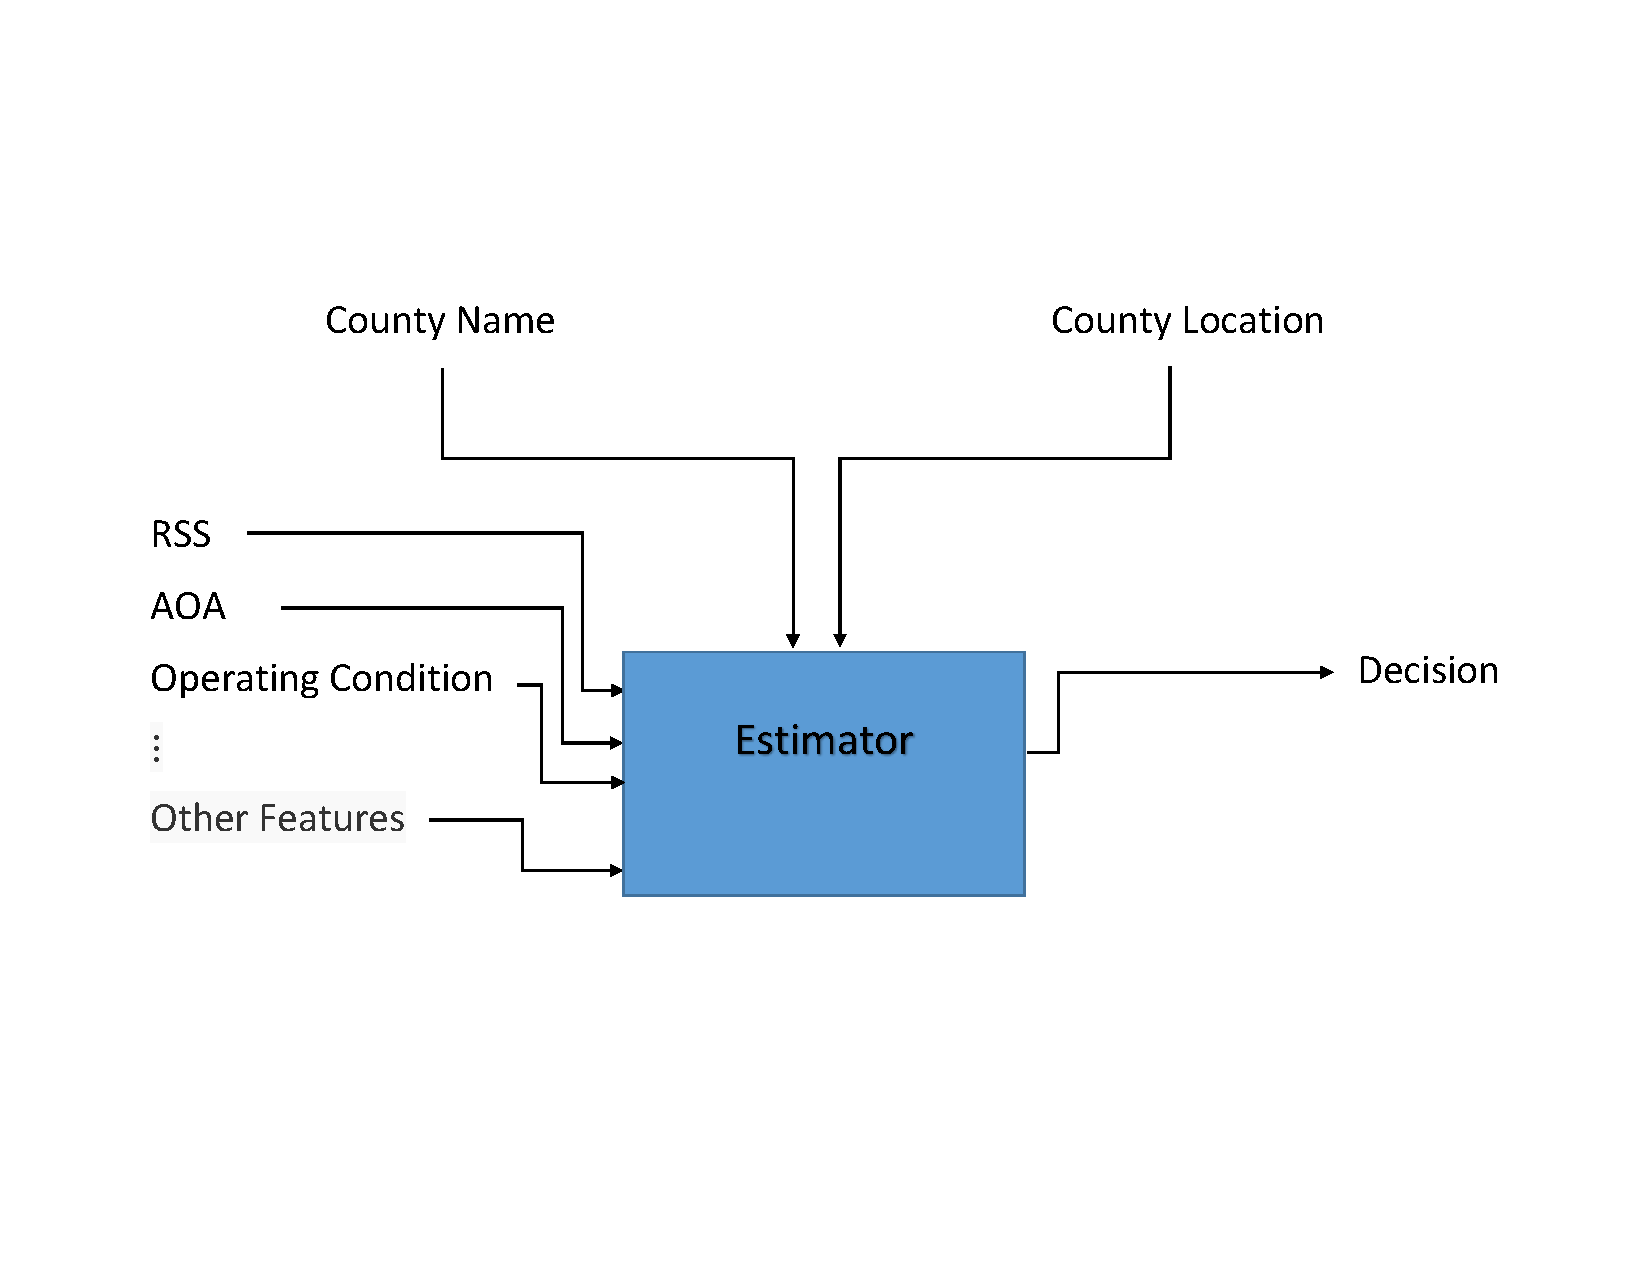
\includegraphics[width=.8\textwidth]{classifier2}
\end{center}
\end{frame}

\subsection{Mathematical Theory}

\begin{frame}
\frametitle{DS Theory: Mathematical Foundation}
Suppose that:
\begin{itemize}
\item{Finite set of all possible mutually exclusive values are denoted as Frame of Discernment, $\Theta$}
\item{$A_1,\dots,A_n$ denote all possible sets within power set $2^\Theta$}
\end{itemize}
\begin{theorem}[Basic Probability Assignment (BPA) $m$]
{$m: 2^\Theta \rightarrow [0,1], \sum\limits_{i=1}^n m(A_i) = 1, m(\emptyset) = 0$}
\end{theorem}
\begin{theorem}[Aggregation of $m_1$ and $m_2$]
{$[m_1 \oplus m_2] = \frac{\sum\nolimits_{A\cap B = y} m_1(A)m_2(B)}{1-\sum\nolimits_{A\cap B = y} m_1(A)m_2(B)}$}
\end{theorem}
\end{frame}

\begin{frame}
\frametitle{Belief and Plausibility}
\begin{itemize}
\item{Let $m(A_i)$ denote BPA mass function for set $A_i$}
\item{Belief represents best case scenario in frame of discernment}
\item{Plausibility represents worst case scenario}
\end{itemize}
\begin{theorem}[Belief of B]
{$Bel(B) = \sum\nolimits_{A_i \subset B} m(A_i)$}
\end{theorem}
\begin{theorem}[Plausibility of B]
{$Pl(B) = 1 - \sum\nolimits_{A_i \cap B = \emptyset} m(A_i)$}
\end{theorem}
\end{frame}

\begin{frame}
\frametitle{Linear Representation}
\begin{itemize}
\item{BPA consists of lower bound, upper bound, and confidence probability}
\end{itemize}
\begin{equation}
m = \begin{bmatrix*}
\ubar{x} & \bar{x} & \mu \end{bmatrix*}
\end{equation}
\begin{itemize}
\item{For all BPAs, expected value can be calculated as}
\end{itemize}
\begin{equation}
Val_{Ex} = \sum\nolimits_{BPAs} 
\begin{bmatrix*} \mu \ubar{x} & \mu \bar{x} \end{bmatrix*}
\end{equation}
\begin{itemize}
\item{An aggregate BPA can be expressed in matrix form as}
\end{itemize}
\begin{equation}
m = \begin{bmatrix*}
m_1 \\
m_2 \\
\vdots \\
m_n \end{bmatrix*}
= \begin{bmatrix*}
\ubar{x}_1 & \bar{x}_1 & \mu_1 \\
\ubar{x}_2 & \bar{x}_2 & \mu_2 \\
\vdots & \vdots & \vdots \\
\ubar{x}_n & \bar{x}_n & \mu_n \\ \end{bmatrix*}
\end{equation}
\end{frame}

\begin{frame}
\frametitle{Data Fusion}
\begin{itemize}
\item{Measurement types (features) consist of RSS, AOA, and operating condition (standby mode)
\begin{equation}
\lambda = \begin{bmatrix*}
\lambda_{RSS} &  \lambda_{AOA} &  \lambda_{SB} \end{bmatrix*}^T
\label{m}
\end{equation}
where
\begin{equation}
\lambda_{RSS} = \begin{bmatrix*}
m_{1,RSS} \\
m_{2,RSS} \\
\vdots \\
m_{n,RSS} \end{bmatrix*},
\lambda_{AOA} = \begin{bmatrix*}
m_{1,AOA} \\
m_{2,AOA} \\
\vdots \\
m_{n,SB} \end{bmatrix*},
\lambda_{SB} = \begin{bmatrix*}
m_{1,SB} \\
m_{2,SB} \\
\vdots \\
m_{n,SB} \end{bmatrix*}
\label{m}
\end{equation}
\begin{equation}
m_i = \begin{bmatrix*}
d_{min} & d_{max} & 1 \end{bmatrix*}, i = 1,2,\dots,n
\label{bpa-d}
\end{equation}}
\end{itemize}
\end{frame}

\begin{frame}[allowframebreaks]
\frametitle{Measurement Types}
\begin{itemize}
\item{RSS $\propto$ $\frac{1}{d^a}$ in general context; $a=2$ in free space}
\end{itemize}
\begin{equation}
RSS = \frac{1}{d^2}
\end{equation}
\begin{itemize}
\item{AOA is determined as}
\end{itemize}
\begin{equation}
 AOA =
  \begin{cases}
   tan^{-1}(\frac{y_n-y_m}{x_n-x_m}) & \text{if } y_n > y_m \text{ and } x_n > x_m \\
   tan^{-1}(\frac{y_n-y_m}{x_n-x_m}) + 180       & \text{if } y_n \neq y_m \text{ and } x_n < x_m \\
   tan^{-1}(\frac{y_n-y_m}{x_n-x_m}) + 360       & \text{if } y_n < y_m \text{ and } x_n > x_m
  \end{cases}
\label{aoa}
\end{equation}
\framebreak
\begin{itemize}
\item{Standby is distance measurement of node in low power (standby) mode from standby node}
\item{Distance is obtained by back calculation of RSS}
\end{itemize}
\begin{equation}
SB = \sqrt{\frac{1}{RSS_{sb}}}
\end{equation}
\begin{equation}
SB = \sqrt{(x_{sb}^2 - x_n^2) + (y_{sb}^2 - y_n^2)}
\end{equation}
\end{frame}

\subsection{Experimental Setup}

\begin{frame}
\frametitle{Overview of First Algorithm}
\begin{figure}[!t]
\centering
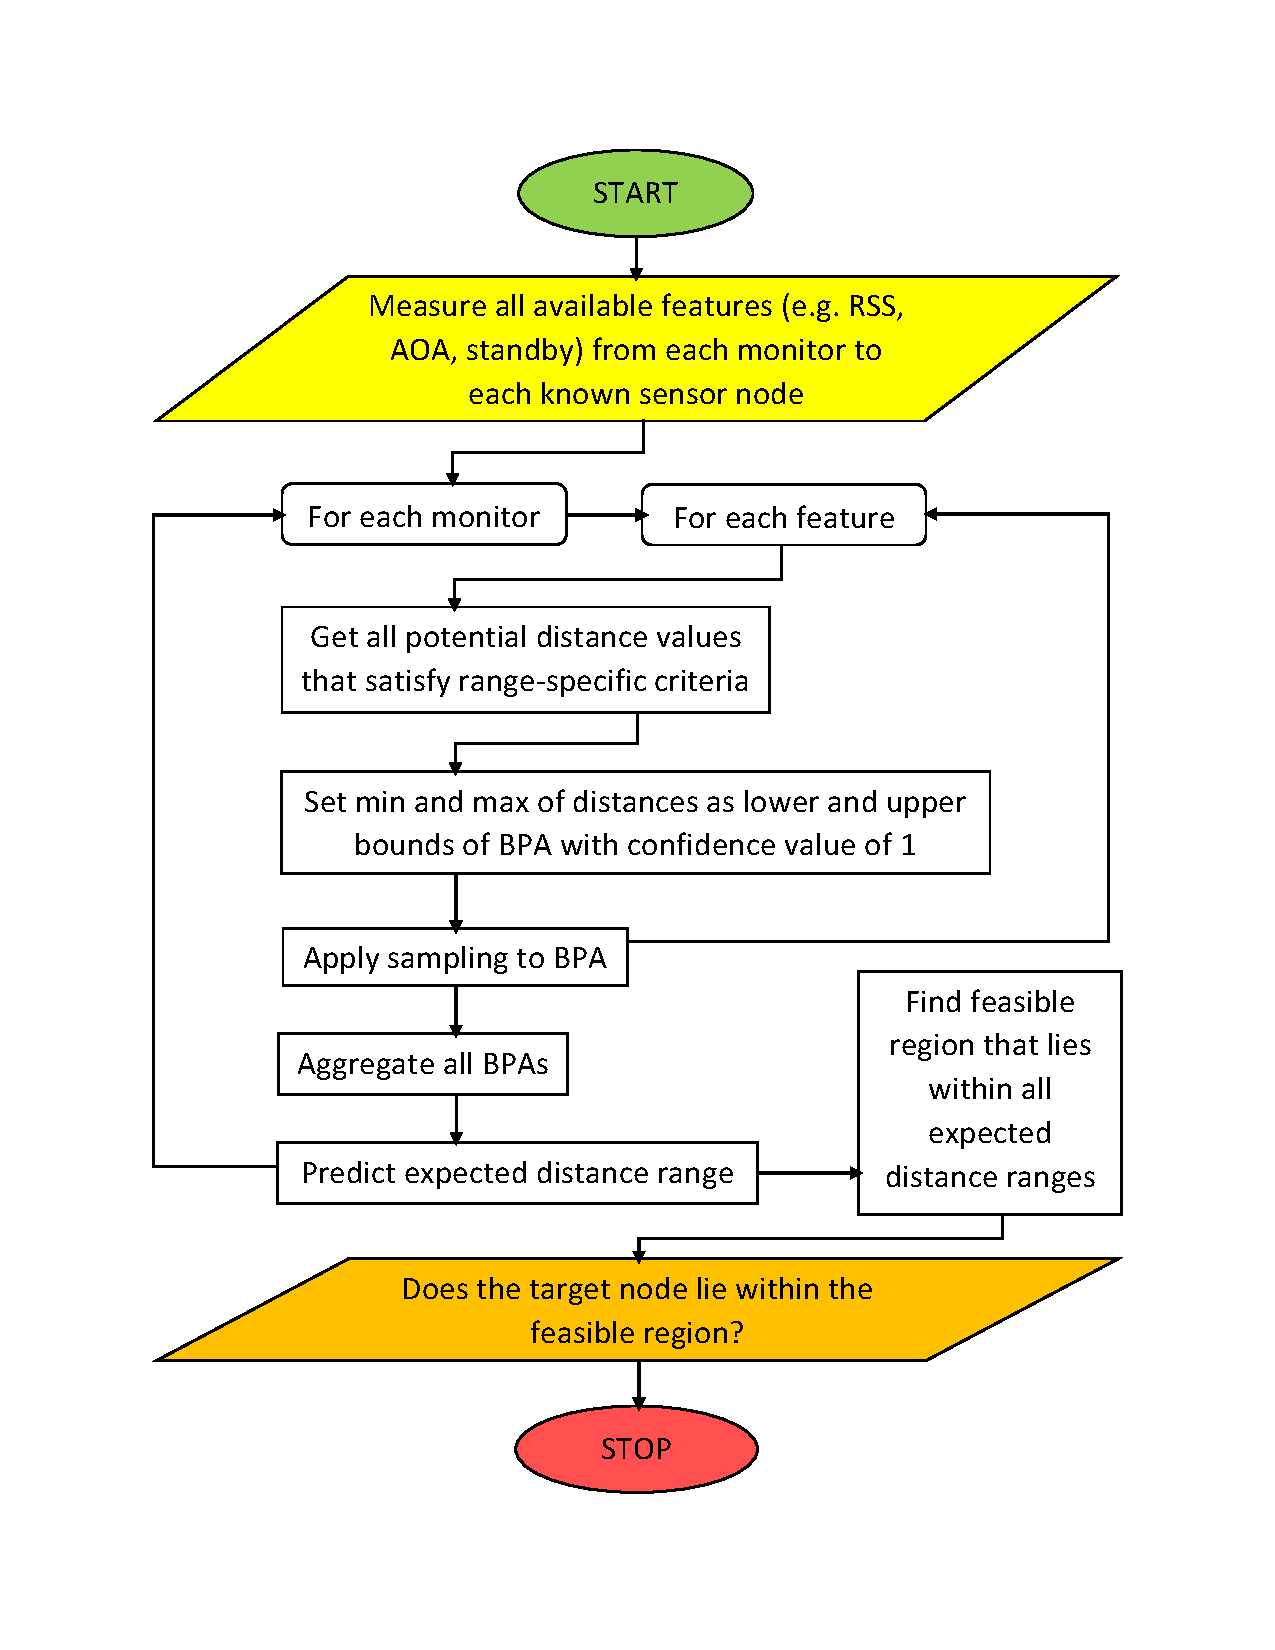
\includegraphics[width=2in]{flowchart1}
\caption{Flowchart of DS localization algorithm.}
\label{dsalg1}
\end{figure}
\end{frame}

\begin{frame}
\frametitle{Algorithm in Execution}
\begin{center}
\includegraphics<1>[width=.85\textwidth]{frame2-0.eps}
\includegraphics<2>[width=.85\textwidth]{frame1-1.eps}
\includegraphics<3>[width=.85\textwidth]{frame1-2.eps}
\includegraphics<4>[width=.85\textwidth]{frame1-3.eps}
\includegraphics<5>[width=.85\textwidth]{frame1-4.eps}
\end{center}
\end{frame}

\begin{frame}[allowframebreaks]
\frametitle{Experimental Setup}
\begin{center}
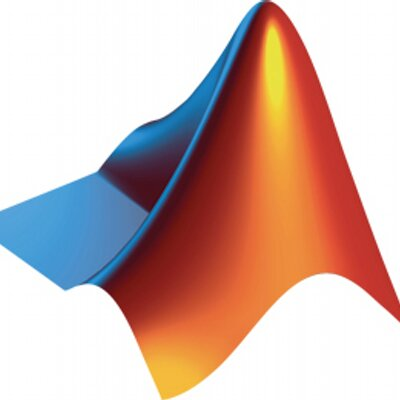
\includegraphics[width=.2\textwidth]{ml}
\end{center}
\begin{itemize}
\item{Software: MATLAB with IPP Toolbox}
\item{Hardware: Quad Core CPU and 8.0 GB RAM}
\item{10 Independent Trials for each feature combination}
\item{100 sensor nodes, 3 anchor nodes, standby node, fusion center}
\end{itemize}
\framebreak
\begin{itemize}
\item{One-to-one mapping between sensor nodes and counties}
\item{RSS range of 20, AOA range of 100, no standby range}
\item{Tested for RSS+SB, RSS+AOA, and RSS+AOA+SB}
\item{10 samples per BPA as inverse normalized distribution}
\item{Zero noise factor and zero anchor node positioning error assumed}
\end{itemize}
\end{frame}

\begin{frame}[allowframebreaks]
\frametitle{Accuracy Calculation}
\begin{itemize}
\item{A decision is made for every combination of county and measurement set}
\item{Decision is either yes (1) or no (0)}
\end{itemize}
\begin{equation}
\begin{bmatrix*}
dec_{11} & dec_{12} & \dots & dec_{1n} \\
dec_{21} & dec_{22} & \dots & dec_{2n} \\
\vdots & \vdots & \ddots & \vdots \\
dec_{n1} & dec_{n2} & \dots & dec_{nn} \end{bmatrix*}
\end{equation}
\framebreak
\begin{itemize}
\item{The results are compared against the ideal decision matrix}
\end{itemize}
\begin{equation}
\begin{bmatrix*}
1 & 0 & \dots & 0 \\
0 & 1 & \dots & 0 \\
\vdots & \vdots & \ddots & \vdots \\
0 & 0 & \dots & 1 \end{bmatrix*}
\end{equation}
\begin{itemize}
\item{Accuracy is calculated by}
\end{itemize}
\begin{equation}
Accuracy = 100*\frac{cells_{matching}}{cells_{total}}
\end{equation}
\end{frame}

\subsection{Results and Discussion}

\begin{frame}
\frametitle{Internal Results}
\begin{table}[!t]
\renewcommand{\arraystretch}{1.3}
\caption{Simulation results.}
\label{table-1}
\centering
$\begin{tabular}{*{3}{l}}
\toprule
Feature Description & Test Accuracy (\%) & Runtime ($\mu$s) \\ \midrule
RSS, SB & 79.97 & 12736.30 \\
RSS, AOA & 78.41 & 12731.71 \\
RSS, AOA, SB & 87.36 & 12731.49 \\ \bottomrule
\end{tabular}$
\end{table}
\end{frame}

\begin{frame}
\frametitle{External Results}
\begin{table}
\renewcommand{\arraystretch}{1.3}
\caption{Comparison of accuracy among different localization techniques.}
\label{compare1}
\centering
$\begin{tabular}{*{6}{l}}
\toprule
Algorithm & PSO & WSLA & WSRA & MLE & DS1 \\
\midrule
Accuracy (\%) & 71 & 90 & 92 & 93 & 87 \\
Runtime ($\mu$s) & 114570 & 7800 & 9700 & NR & 12733 \\
\bottomrule
\end{tabular}$
\end{table}
\end{frame}

\section{Second Method: Plausibility}

\subsection{Introduction and Background}

\begin{frame}
\frametitle{Second Proposed Algorithm}
\begin{itemize}
\item{Does the set of measurements belong to the county?}
\item{Which county most closely matches the set of measurements?}
\end{itemize}
\begin{center}
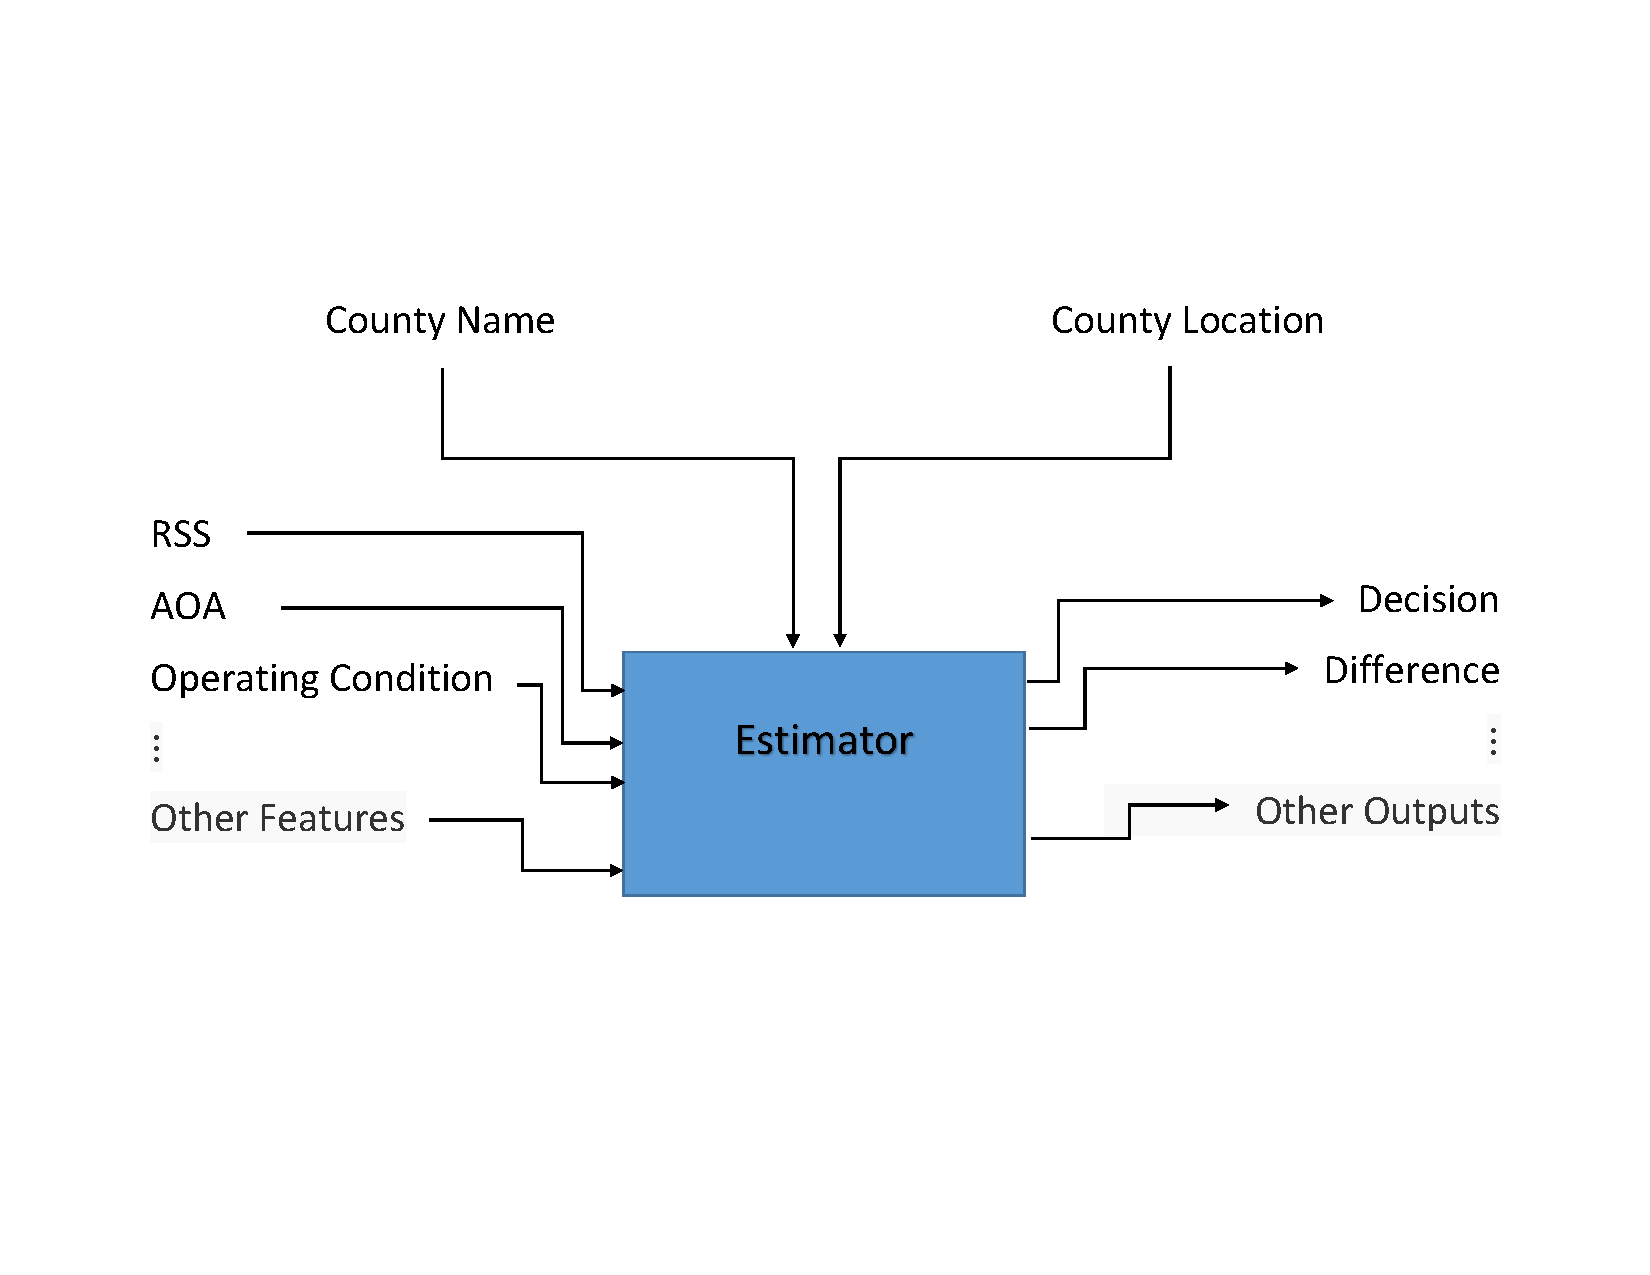
\includegraphics[width=.8\textwidth]{classifier}
\end{center}
\end{frame}

\subsection{Mathematical Theory}

\begin{frame}[allowframebreaks]
\frametitle{Formation of Belief}
\begin{itemize}
\item{Recall that an aggregate BPA can be expressed as}
\end{itemize}
\begin{equation}
m = \begin{bmatrix*}
m_1^u \\
m_2^u \\
\vdots \\
m_n^u \end{bmatrix*}
= \begin{bmatrix*}
\ubar{x}_1^u & \bar{x}_1^u & \mu_1^u \\
\ubar{x}_2^u & \bar{x}_2^u & \mu_2^u \\
\vdots & \vdots & \vdots \\
\ubar{x}_n^u & \bar{x}_n^u & \mu_n^u \\ \end{bmatrix*}
\label{m-1}
\end{equation}
\begin{itemize}
\item{Superscript $u$ denotes that $\bar{x}_1^u < \bar{x}_2^u < \dots < \bar{x}_n^u$}
\framebreak
\item{Then belief can be formed as
\begin{equation}
Bel = \begin{bmatrix*}
\bar{x}_1^u & \mu_{1,new}^u \\
\bar{x}_2^u & \mu_{2,new}^u \\
\vdots & \vdots \\
\bar{x}_n^u & \mu_{n,new}^u \end{bmatrix*}
\end{equation}
where 
\begin{equation}
\mu_{1,new}^u = \mu_1^u
\label{mu1l}
\end{equation}
\begin{equation}
\mu_{2,new}^u = \mu_2^l+\mu_{1,new}^u
\label{mu2l}
\end{equation}
\begin{equation}
\mu_{n,new}^u = \mu_n^u+\mu_{(n-1),new}^u
\label{munl}
\end{equation}}
\end{itemize}
\end{frame}

\begin{frame}[allowframebreaks]
\frametitle{Formation of Plausibility}
\begin{itemize}
\item{Now suppose $m$ is rearranged and $m_{1}^{u}, m_{2}^{u},\dots, m_{n}^{u}$ are renamed such that}
\end{itemize}
\begin{equation}
m = \begin{bmatrix*}
m_1^l \\
m_2^l \\
\vdots \\
m_n^l \end{bmatrix*}
= \begin{bmatrix*}
\ubar{x}_1^l & \bar{x}_1^l & \mu_1^l \\
\ubar{x}_2^l & \bar{x}_2^l & \mu_2^l \\
\vdots & \vdots & \vdots \\
\ubar{x}_n^l & \bar{x}_n^l & \mu_n^l \\ \end{bmatrix*}
\label{mu}
\end{equation}
\begin{itemize}
\item{Superscript $l$ denotes that $\ubar{x}_1^u < \ubar{x}_2^u < \dots < \ubar{x}_n^u$}
\framebreak
\item{Then plausibility can be formed as
\begin{equation}
Pl = \begin{bmatrix*}
\ubar{x}_1^l & \mu_{1,new}^l \\
\ubar{x}_2^l & \mu_{2,new}^l \\
\vdots & \vdots \\
\ubar{x}_n^l & \mu_{n,new}^l \end{bmatrix*}
\label{m}
\end{equation}
\noindent where
\begin{equation}
\mu_{1,new}^l = \mu_1^l
\label{mu1u}
\end{equation}
\begin{equation}
\mu_{2,new}^l = \mu_2^l+\mu_{1,new}^l
\label{mu2u}
\end{equation}
\begin{equation}
\mu_{n,new}^l = \mu_n^l+\mu_{(n-1),new}^l
\label{munu}
\end{equation}}
\end{itemize}
\end{frame}

\begin{frame}
\frametitle{Overview of Second Algorithm}
\begin{figure}[!t]
\centering
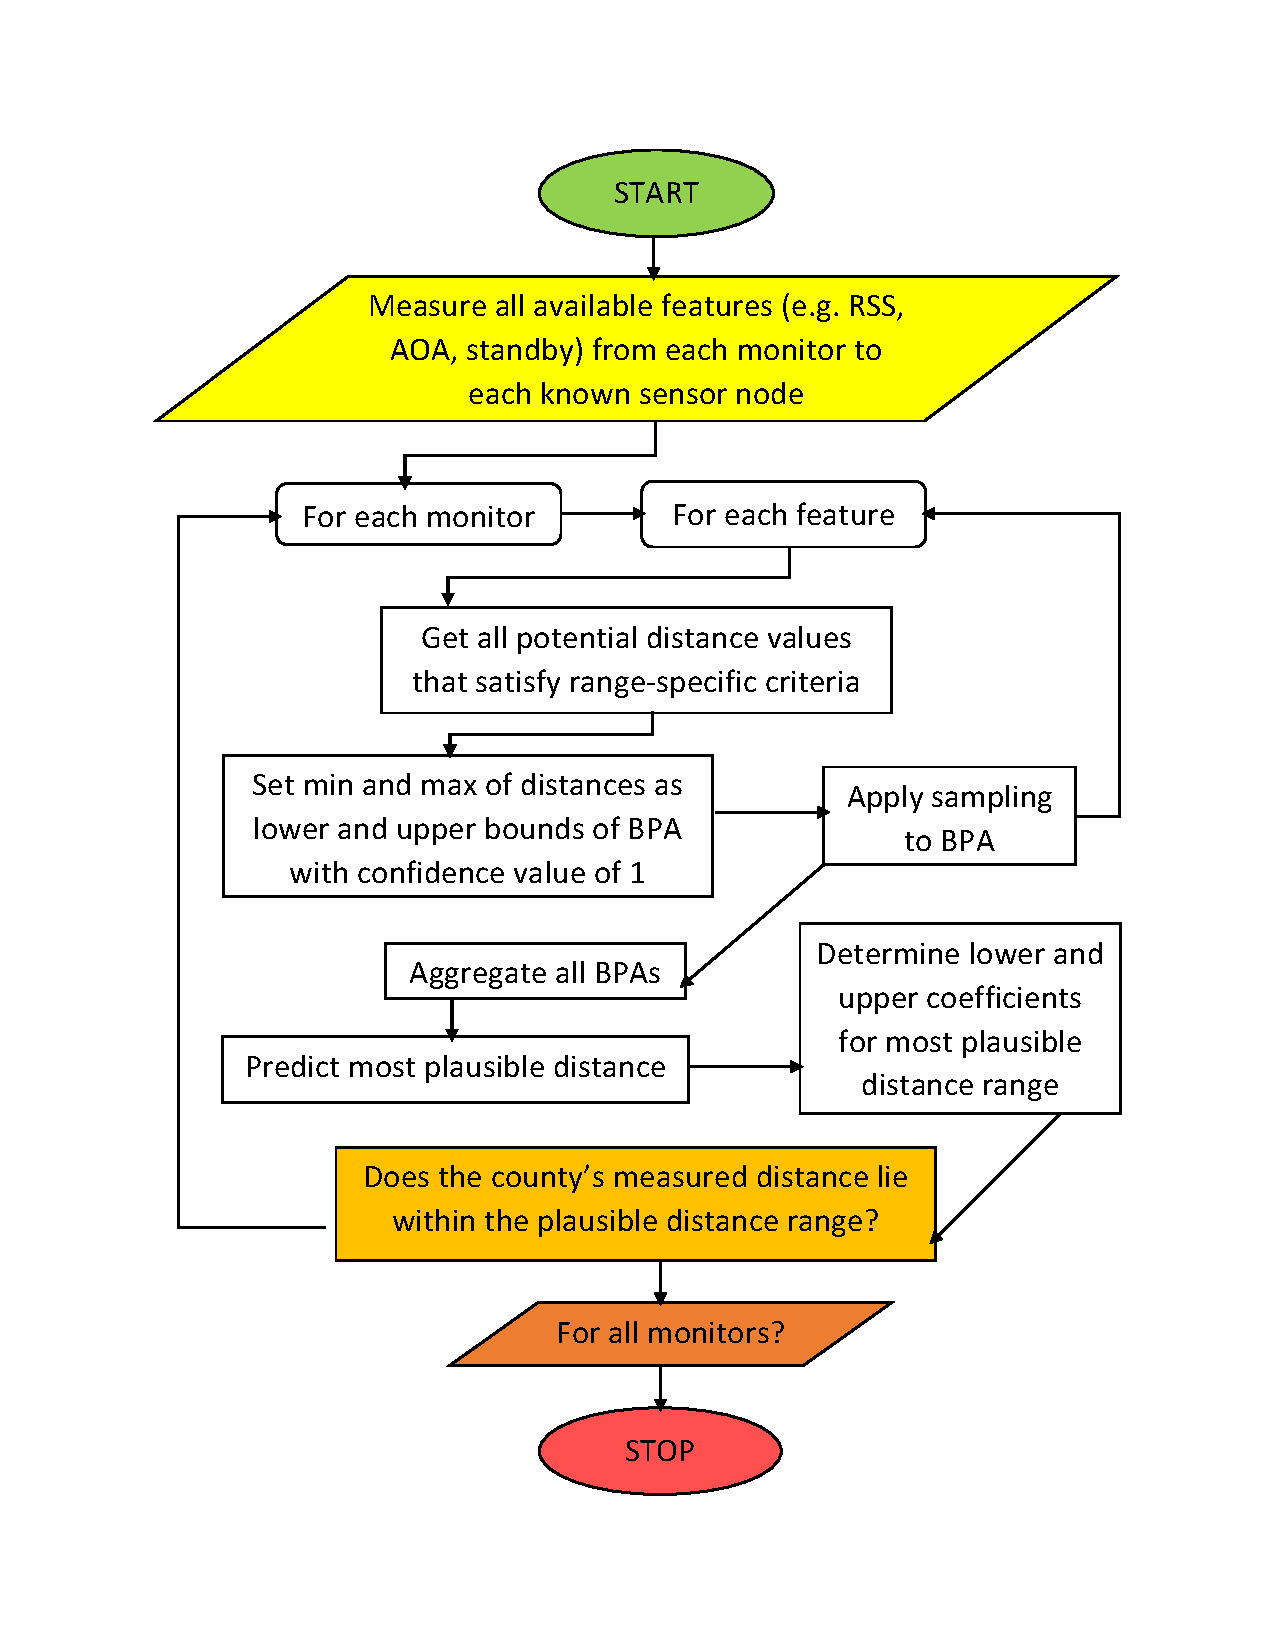
\includegraphics[width=2in]{flowchart2}
\caption{Flowchart of DS localization algorithm}
\label{dsalg2}
\end{figure}
\end{frame}
\subsection{Experimental Setup}

\begin{frame}
\frametitle{Algorithm in Execution}
\begin{center}
\includegraphics<1>[width=.85\textwidth]{frame2-0.eps}
\includegraphics<2>[width=.85\textwidth]{frame2-1.eps}
\includegraphics<3>[width=.85\textwidth]{frame2-2.eps}
\includegraphics<4>[width=.85\textwidth]{frame2-3.eps}
\includegraphics<5>[width=.85\textwidth]{frame2-4.eps}
\end{center}
\end{frame}

\begin{frame}
\frametitle{Determination of Optimal Distance Range}
\begin{center}
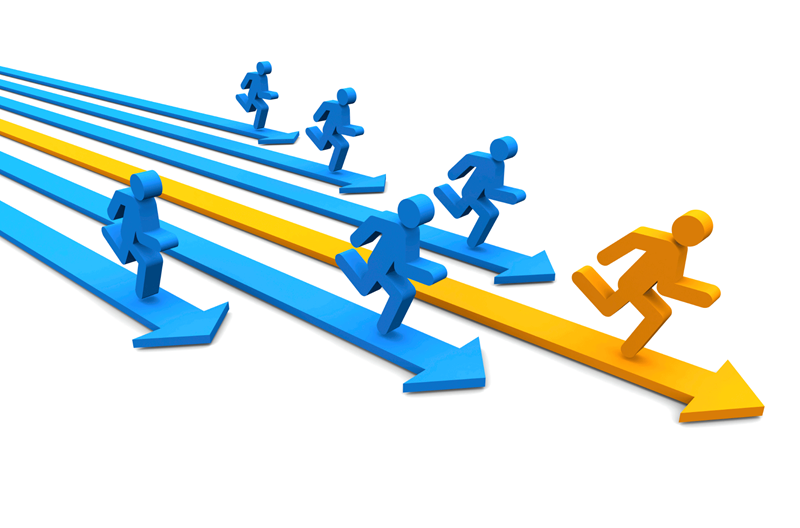
\includegraphics[width=.25\textwidth]{train}
\end{center}
\begin{itemize}
\item{Need upper and lower weights to determine distance range that yields most optimal accuracy}
\item{Training is one-time occurrence not essential to DS Theory}
\item{Candidate upper bounds are 1.1, 1.3, 1.5, 1.7, and 1.9}
\item{Candidate lower bounds are 0.2, 0.45, 0.7, and 0.95}
\item{Iterative training consists of 30 independent trials per feature set}
\end{itemize}
\end{frame}

\begin{frame}
\frametitle{Changes in Experimental Setup}
\begin{center}
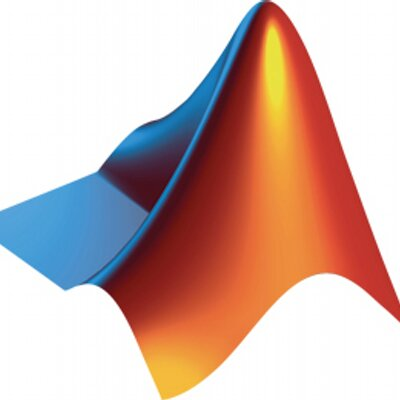
\includegraphics[width=.2\textwidth]{ml}
\end{center}
\begin{itemize}
\item{Tested for both 2 and 3 active anchor nodes}
\item{AOA range of .002}
\item{Inverses of feature values compared with range values}
\item{Tested for every feature combination in which RSS is active}
\item{(Actual distance - predicted distance) of <-1.5 not considered}
\end{itemize}
\end{frame}

\begin{frame}
\frametitle{Three Types of Accuracy Calculation}
\begin{center}
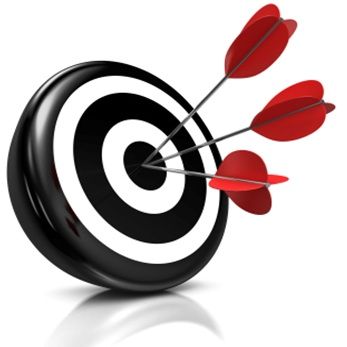
\includegraphics[width=.2\textwidth]{acc}
\end{center}
\begin{itemize}
\item{\textbf{Full Accuracy}

Based on all possible combinations of measurement sets and counties}
\item{\textbf{Short Accuracy}

Based only on all possible correct combinations}
\item{\textbf{Matching Accuracy}

Based on county matches for all measurement sets}
\end{itemize}
\end{frame}

\begin{frame}
\frametitle{Full Accuracy Calculation}
\begin{itemize}
\item{Decision matrix
\begin{equation}
\begin{bmatrix*}
dec_{11} & dec_{12} & \dots & dec_{1n} \\
dec_{21} & dec_{22} & \dots & dec_{2n} \\
\vdots & \vdots & \ddots & \vdots \\
dec_{n1} & dec_{n2} & \dots & dec_{nn} \end{bmatrix*}
\end{equation}
is compared against ideal matrix
\begin{equation}
\begin{bmatrix*}
1 & 0 & \dots & 0 \\
0 & 1 & \dots & 0 \\
\vdots & \vdots & \ddots & \vdots \\
0 & 0 & \dots & 1 \end{bmatrix*}
\end{equation}
for all combinations of measurement sets and counties}
\end{itemize}
\end{frame}

\begin{frame}
\frametitle{Short Accuracy Calculation}
\begin{itemize}
\item{Decision matrix based only on correct combinations
\begin{equation}
\begin{bmatrix*}
dec_1 & dec_2 & \dots & dec_n
\end{bmatrix*}
\end{equation}}
\item{Ideal matrix
\begin{equation}
\begin{bmatrix*}
1 & 1 & \dots & 1
\end{bmatrix*}
\end{equation}}
\end{itemize}
\end{frame}

\begin{frame}
\frametitle{Matching Accuracy Calculation}
\begin{itemize}
\item{Matching matrix based on all possible feature sets
\begin{equation}
\begin{bmatrix*}
match_1 & match_2 & \dots & match_n
\end{bmatrix*}
\end{equation}}
\item{Ideal matrix
\begin{equation}
\begin{bmatrix*}
1 & 2 & \dots & n
\end{bmatrix*}
\end{equation}}
\end{itemize}
\end{frame}

\subsection{Results and Discussion}

\begin{frame}
\frametitle{Accuracy Results under Iterative Weight Training}
\begin{figure*}\centering
\subfloat[Full Accuracy\label{fullacc}]
        {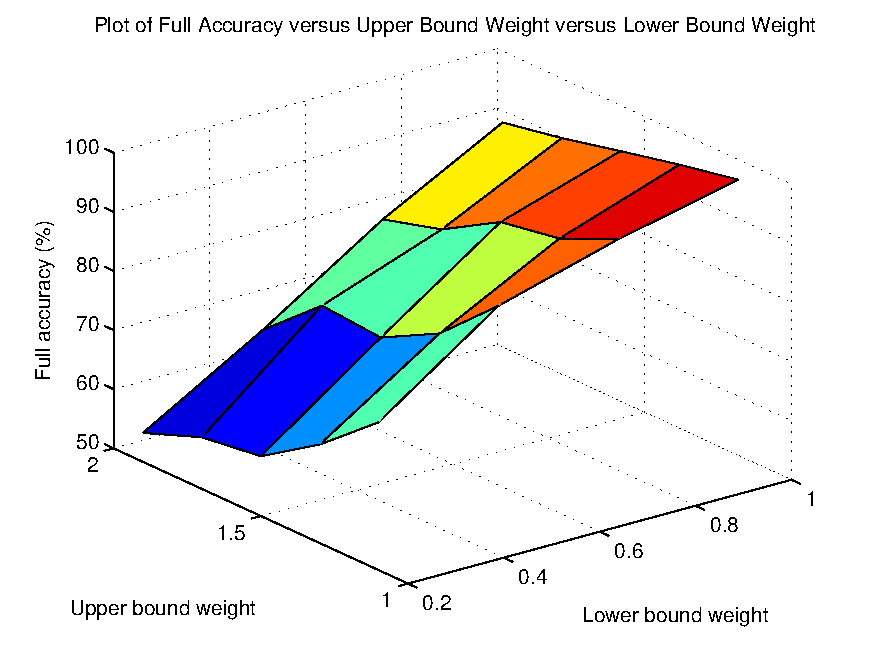
\includegraphics[width=0.3\textwidth]{longacc}}
    \hfill
\subfloat[Short Accuracy \label{shortacc}]
         {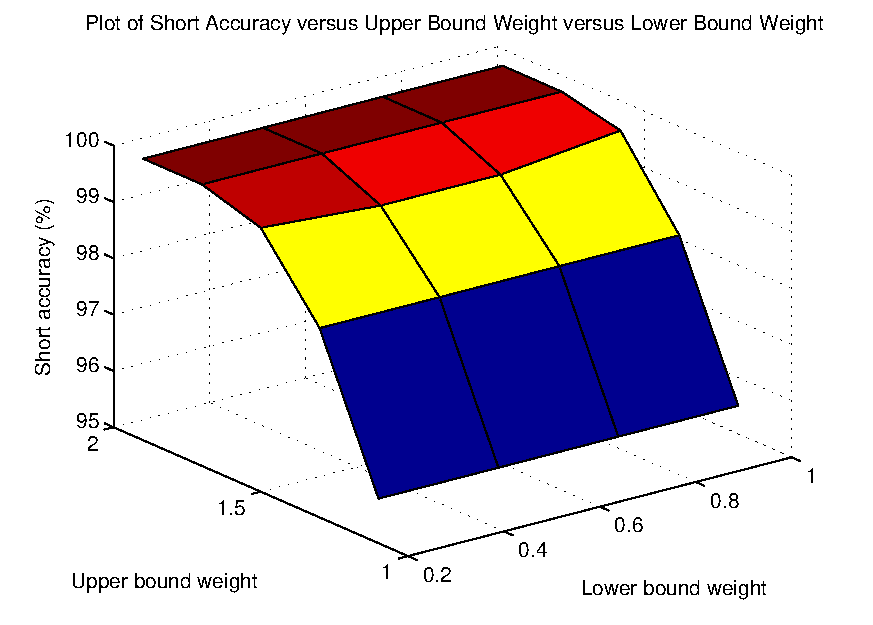
\includegraphics[width=0.3\textwidth]{shortacc}}
\hfill
\subfloat[Matching Accuracy \label{matchacc}]
         {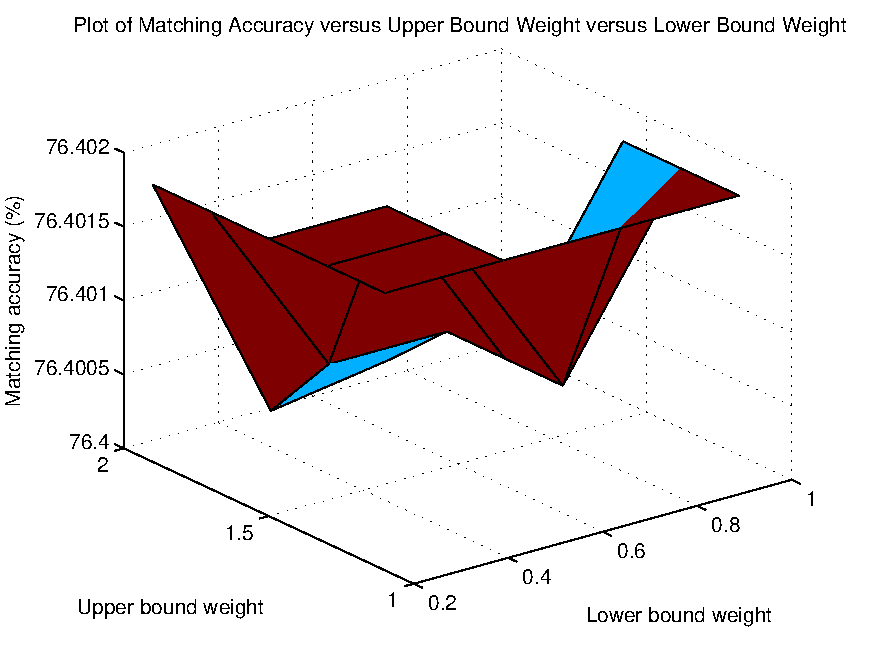
\includegraphics[width=0.3\textwidth]{matchacc}}
    \hfill
\subfloat[Average Accuracy \label{avgacc}]
        {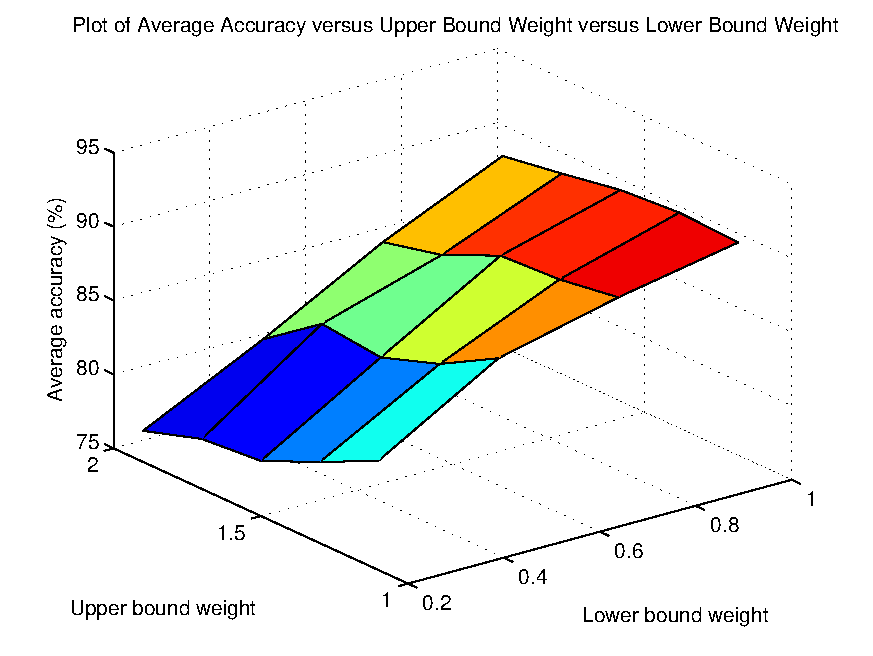
\includegraphics[width=0.3\textwidth]{avg}}
    \label{train-acc}
    \end{figure*}
\end{frame}

\begin{frame}
\frametitle{Internal Results: Accuracy}
\begin{table}[!t]
\renewcommand{\arraystretch}{1.3}
\caption{Simulation results for two-monitor and three-monitor WSNs.}
\label{table_example}
\centering
\resizebox{\textwidth}{!}
{\begin{tabular}{*{7}{l}|*{2}{l}}
\toprule
Accuracy  & \multicolumn{2}{l}{Full (\%)} & \multicolumn{2}{l}{Short (\%)} & \multicolumn{2}{l|}{Match (\%)} & \multicolumn{2}{l}{Average (\%)} \\
Monitors & 2 & 3 & 2 & 3 & 2 & 3 & 2 & 3 \\ \midrule
RSS & 97.04 & 97.49 & 97.20 & 98.50 & 56.17 & 66.64 & 83.47 & 87.54 \\
RSS, SB & 97.00 & 97.43 & 100.0 & 100.0 & 94.58 & 96.07 & 97.19 & 97.83 \\
RSS, AOA & 97.03 & 97.47 & 98.13 & 98.97 & 57.81 & 67.29 & 84.33 & 87.92 \\
RSS, AOA, SB & 97.01 & 97.44 & 100.0 & 100.0 & 92.52 & 94.21 & 96.51 & 97.22 \\ \bottomrule
\end{tabular}}
\end{table}
\end{frame}

\begin{frame}
\frametitle{Internal Results: Runtime}
\begin{table}[!t]
\renewcommand{\arraystretch}{1.3}
\caption{Runtime results for two-monitor and three-monitor WSNs.}
\label{table_run_time}
\centering
$\begin{tabular}{*{3}{l}}
\toprule
Runtime (ms) & 2 Monitors & 3 Monitors\\ \midrule
Total & 787478.00 & 1375261.00 \\
Per Feature Set & 196869.00 & 343815.20 \\
Per Iteration & 17.20 & 30.03 \\
Per Node & 0.160 & 0.281 \\ 
\bottomrule
\end{tabular}$
\end{table}
\end{frame}

\begin{frame}
\frametitle{External Results}
\begin{table}
\renewcommand{\arraystretch}{1.3}
\caption{Comparison of accuracy among different localization techniques.}
\label{compare2}
\centering
$\begin{tabular}{*{7}{l}}
\toprule
Algorithm & PSO & WSLA & WSRA & MLE & DS1 & DS2 \\
\midrule
Accuracy (\%) & 71 & 90 & 92 & 93 & 87 & 97 \\
Runtime ($\mu$s) & 114570 & 7800 & 9700 & NR & 12733 & 281 \\
\bottomrule
\end{tabular}$
\end{table}
\end{frame}

%------------------------------------------------

\section{Conclusive Remarks}

\begin{frame}
\frametitle{Publications}
Colin Elkin, Rajika Kumarasiri, and Vijay Devabhaktuni, ``A novel approach to localization in wireless sensor networks using Dempster-Shafer evidence theory,'' {\it Expert Systems with Applications} (Under review).
\end{frame}

\begin{frame}
\frametitle{Conclusions}
\begin{itemize}
\item{Dempster-Shafer Evidence Theory was introduced for the first time to the area of WSN localization}
\item{Expected value function generates good accuracy but with high computational cost}
\item{Plausibility function generates great accuracy at low computational cost}
\item{Variety of applications in time-critical WSN localization will be greatly enhanced with these novel algorithms}
\end{itemize}
\end{frame}

\begin{frame}
\frametitle{Future Work}
\begin{itemize}
\item{Fusion of DS Theory with Support Vector Machines}
\item{DS Theory as Meta-Learning Component for Data Mining}
\item{Enhance Training of Upper and Lower Bound Coefficients}
\end{itemize}
\end{frame}

\begin{frame}
\frametitle{Acknowledgements}
\begin{itemize}
\item{Dr.~Vijay Devabhaktuni}
\item{Dr.~Mansoor Alam, Dr.~Richard Molyet, and Dr.~Hong Wang}
\item{NSF, EECS Department, and ET Department}
\item{All attendees here today}
\item{Rajika Kumarasiri, Hem Regmi, and Arushi Gupta}
\item{Colleagues at NE 2033 \& 2042}
\item{My family and friends, both near and far}
\end{itemize}
\end{frame}

\begin{frame}
\frametitle{Thank you}
\Huge{\centerline{Any Questions?}}
\end{frame}

%----------------------------------------------------------------------------------------

\end{document} 